\documentclass[12pt]{article}
\usepackage{amsmath}
\usepackage{amsfonts}
\usepackage{bm}
\usepackage{color}
\usepackage{graphicx}
\definecolor{lyellow}{rgb}{0.97,0.94,0.8}
\definecolor{gray}{rgb}{0.4,0.4,0.4}

%\renewcommand{\baselinestretch}{1.2}

\textwidth 15.5cm
\textheight 22.5cm
\topmargin  0.0cm
\oddsidemargin -0cm
\evensidemargin -0cm
%\pagestyle{empty}

%\partopsep -33pt
%\parsep 0pt
%\topskip -33pt
%\parskip 33pt


\newcommand{\lfrac}[2]{{\displaystyle\frac{{#1}}{{#2}}}}
\newcommand{\ffrac}[2]{{\textstyle\frac{{#1}}{{#2}}}}
\newcommand{\half}{\ffrac{1}{2}}



\newcommand{\I}{\mathrm{i}}
%\newcommand{\bld}[1]{\boldsymbol{#1}}
\newcommand{\cond}{\mbox{\rule[-0.5em]{.1mm}{1.2em}}}

%\renewcommand{\baselinestretch}{0.9}
\renewcommand{\topfraction}{0.8}
\renewcommand{\textfraction}{0.2}
\renewcommand{\floatpagefraction}{0.8}

\newcounter{denselistcounter}
\newenvironment{denselist}[1]
{ \begin{list}
  {#1{denselistcounter})}{\usecounter{denselistcounter}
  \setlength{\topsep}{-0pt}
  \setlength{\partopsep}{-0pt}
  \setlength{\itemsep}{-0pt}
  \setlength{\parsep}{-0pt}
  \setlength{\labelwidth}{6pt}
  \setlength{\labelsep}{4pt}
  \setlength{\leftmargin}{20pt}
  \setlength{\rightmargin}{20pt}
  }
}
{\end{list}}

\newcommand{\Bp}{\mathcal{B}_0}
\newcommand{\Bm}{\mathcal{B}_1}
\newcommand{\PGR}[1]{{\color{blue} #1}}

\begin{document}

\title{Trend with cutoff energy}
\author{Discussion file: FAU -- MSU}
\date{Started: 13 July 2024}
\maketitle

We study the trend of pairing energy with pairing cutoff for different
folding widths. Test case is $^{120}$Sn computed with UNEDF1 and
volume pairing. The pairing strength is tuned for each folding width
such that all cases have about the same pairing energy for the starting
cutoff 15 MeV. 

\bigskip

\centerline{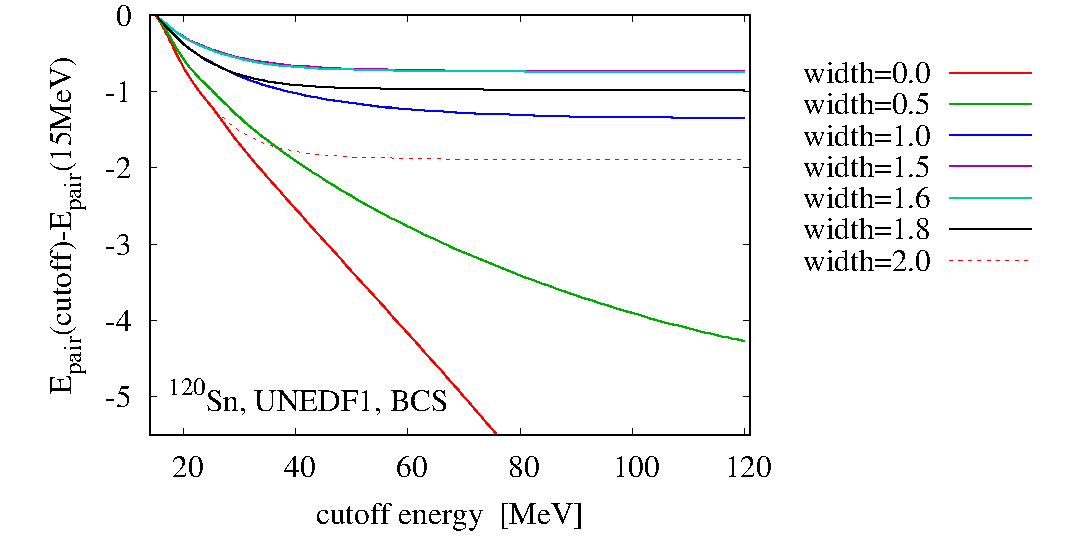
\includegraphics[width=0.99\linewidth]{varycut_BCS}}

\bigskip

The above figure shows the evolution of pairing energy with cutoff
energy shifted such that all start at zero energy (the actual value is
about -20 MeV). Zero width (red line) is a straight line of ever
increasing pairing. The width 0.5 MeV bends the curve to some
convergence which, however, is not in reach for the considered window
of cutoff energies. Larger widths show all nice convergence. The
changes shrink with increasing width up to 1.5 MeV width. Then the
trend turns and the overall changes increase again. This turn around
has yet to be understood. But the overall change does not tell
anything about the speed of convergence. This will be discussed in the
next figure.


\bigskip

\centerline{\includegraphics[width=0.99\linewidth]{varycutn_BCS}}

\bigskip

To compare the speed of convergence, we scale the results all the same
way as
$(E_\mathrm{pair}(E_\mathrm{cut})-E_\mathrm{pair}(15\mathrm{MeV}))/E_\mathrm{pair}(120\mathrm{MeV})$. 
The above figure shows the result. There we see a monotonous
increase in in speed with increasing folding width. But, again, the
improvements slow down above a width of 1.5 MeV. This seems at the
moment an optimal value concerning changes of pairing energy and speed
of convergence.



\end{document}
